\section{Accelerating t-SNE}

The original t-SNE algorithm is not very fast. Its runtime is $\mathcal{O}(n^2)$, which quickly becomes infeasible for datasets with $100,000$ or more points \textcolor{red}{check the exact number}. In this section, we will give an overview of the two most popular methods proposed to speed up the algorithm. 

\subsection{Barnes-Hut t-SNE}
This method uses tree-bases algorithms to speed up t-SNE and was proposed by van der Maaten in 2014 \cite{vdMaa14}. 

\begin{itemize}
    \item the gradient of the t-SNE loss function (KLD) has a natural interpretation as an $N$-body system in which all of the $N$ points in the low-dimensional embedding exert forces on each other. We then need to compute the resultant force on each of the points
\end{itemize}
We start by recalling the gradient of the t-SNE cost function: 
\begin{equation}
    \frac{\partial C}{\partial y_i} = 4 \sum_{j \neq i} (p_{ij} - q_{ij}) q_{ij} Z (y_i - y_j)
\end{equation}
with normalization term $Z = \sum_{k \neq l} (1+ \norm{y_k - y_l}^2 )^{-1}$. Notice that we can split the gradient into two parts 
\begin{equation}
    \frac{\partial C}{\partial y_i} = 4 (F_{\text{attr}} + F_{\text{rep}}) = 4 \left( \sum_{j \neq i } p_{ij} q_{ij} Z (y_i - y_j) - \sum_{j \neq i} q_{ij}^2 Z (y_i - y_j) \right) 
\end{equation}
where $F_{\text{attr}}$ denotes the sum of all attractive forces and $F_{\text{rep}}$ the sum of all repulsive forces. 

This next explanation is taken from \cite{LinStei22}. \textcolor{red}{TODO: maybe move explanation to the EE section, I think it would make sense there, or maybe do a whole section on the dynamical systems viewpoint}

Why does it make sense to call these attractive and repulsive forces? Since we want to minimize the cost function, we perform gradient descent and step in the direction of the negative gradient, so we consider the term
\begin{equation}
   - \frac{1}{4} \frac{\partial C}{\partial y_i} = \sum_{j \neq i } p_{ij} q_{ij} Z (y_j - y_i) - \sum_{j \neq i} q_{ij}^2 Z (y_j - y_i).  
\end{equation}
The first term is considered the attractive term, since it moves the point $y_i$ towards a weighted average of the other $y_i$. 
The weights $p_{ij} q_{ij} Z$ are bigger if the two points are close to each other (both in the low- and high-dimensional space). 
The second term has the opposite sign and thus pushes $y_i$ away from a weighted average of the other points. This time, however, the weights only depend on the closeness of points in the low-dimensional space. 
Put together, this means that the attractive term attracts points that are actually meant to be with each other (based on their similarity in the high-dimensional space) and the repulsive term pushes points apart that get too close in the embedding space, regardless of their real similarity. 

\subsubsection{Approximating Attractive Forces}
Computing the attractive force is not too expensive computationally, if we approximate input similarities and use vantage-point trees. Recall that input similarities $p_{ij}$ are computed based on a Gaussian kernel. 
Thus, $p_{ij}$ values corresponding to dissimilar input objects $x_i$ and $x_j$ are very small. 
So, it makes sense to develop a sparse approximation for the $p_{ij}$. Instead of computing $n^2$ pairwise similarities, we focus on the $\lfloor 3 \kappa \rfloor$ nearest neighbors of each of the $n$ input objects only, where $\kappa$ denotes the perplexity. We denote the nearest neighbor set of $x_i$ by $\mathcal{N}_i$. 

The similarities are thus given by 
\begin{equation}
    p_{j|i} = \begin{cases}
    \frac{\exp(-\norm{x_i - x_j}^2) / 2 \sigma_i^2}{\sum_{k \in \mathcal{N}_i} \exp(-\norm{x_i - x_k}^2) / 2 \sigma_i^2} & \text{ if } j \in \mathcal{N}_i \\
    0  & \text{ otherwise}
    \end{cases}
\end{equation}
which are again symmetrized then. 

We can find the nearest neighbor sets $\mathcal{N}_i$ in $\mathcal{O}(u n \log n)$ time by building a data structure called a vantage-point tree and performing nearest neighbor search with its help. For details, see \cite{vdMaa14}. 

\textcolor{red}{TODO: maybe say more about vantage-point trees here?}

\subsubsection{Approximating Repulsive Forces}
Naively computing the repulsive forces is not a good idea. It would be in $\mathcal{O}(n^2)$. 
Using the Barnes-Hut algorithm however, this can be sped up to $\mathcal{O}(n \log n)$. 
The algorithm relies on the observation that the repulsive forces exerted between two small groups of points are very similar whenever these two groups are relatively far away from each other. 
More precisely, if we consider points $y_i, y_j$ and $y_k$ with $\norm{y_i - y_j} \approx \norm{y_i - y_k} \gg \norm{y_j - y_k}$, then the contributions of $y_j$ and $y_k$ to $F_{\text{rep}, i}$ will be roughly equal. 

To take advantage of this fact, the Barnes-Hut algorithm constructs a data structure known as a quadtree (or for three-dimensional embeddings an octtree). Once we have built a quadtree on the current embedding, we traverse it via depth-first search and decide at every node of the quadtree, whether the corresponding cell can be used as a summary for the contributions to $F_{\text{rep}}$ of all points in the cell or if we need to go deeper. 

\textcolor{red}{Maybe insert a picture of a Quadtree here? But I am not sure how much to write about Barnes-Hut really...}

\subsection{Fast Interpolation-Based t-SNE}
As observed in \cite{KoBe19SingleCell}, the Barnes-Hut implementation of t-SNE, while faster than the originally proposed algorithm, still becomes provibitively slow for datasets with $n \gg 100,000$. 
The FFT accelerated, fast interpolation-based version of t-SNE proposed by Linderman et. al. in 2019 \cite{Lin19} attempts to further speed up the computation of t-SNE embeddings with a special view towards applications in the analysis of single-cell RNA-seq data, which keeps growing and datasets often have north of 1 million datapoints. 

% algorithm pseudocode here
\begin{algorithm}[H]
    \caption{FFT-accelerated Interpolation-based t-SNE (FIt-SNE)}
    \label{alg:fit-sne}
    \KwIn{embedding points $\{y_i\}_{i=1}^N$, interpolation coefficients $\{q_i\}_{i=1}^N$, number of intervals $N_{\text{int}}$, interpolation points per interval $p$}
    \KwOut{$\varphi(y_i) = \sum_{i=1}^N K(y_i, y_j) q_j$ for $i=1, \dots, N$}


    For every interval $I_l$, form $p$ equispaced nodes $\tilde{y}_{j, l} = 1/(2N_{\text{int}}p) + \frac{j-1 + (l-1)p}{N_{\text{int}}p}$ for $j=1,\dots,p$. 

    \For{$I = 1$ \KwTo $N_{\text{int}}$}{
        Compute the coefficients $w_{m,l}$ given by 

        \[
            w_{m,l} = \sum_{y_i \in I_l} L_{m, \tilde{y}^l}(y_i) q_i, \text{      } m=1,\dots,p
        \]
    }

    Use FFT to compute values of $v_{m,n}$ given by 

        \[
            \begin{pmatrix}
                v_{1,1} & v_{2,1} & \dots & v_{p, N_{\text{int}}}
            \end{pmatrix}^T = \tilde{K} \begin{pmatrix}
                w_{1,1} & w_{2,1} & \dots & w_{p, N_{\text{int}}}
            \end{pmatrix}^T
        \]
    where $\tilde{K}$ is the Toeplitz matrix given by $\tilde{K}_{ij} = K(\tilde{y_i}, \tilde{y_j})$, $i, j = 1, \dots, N_{\text{int}}p$.
    
    \For{$I = 1$ \KwTo $N_{\text{int}}$}{
        Compute $\varphi(y_i)$ at all points $y_i \in I_l$ via 

        \[
            \varphi(y_i) = \sum_{j=1}^p L_{j, \tilde{y}^l}(y_i) v_{j,l}
        \]
    }

\end{algorithm}

\subsection{Comparing Barnes-Hut and FIt-SNE}
When comparing the two methods, we only see minor differences in the embedding. 
However, the FIt-SNE version is many times faster than Barnes-Hut t-SNE, which is why we will be using FIt-SNE in all of our experiments going forward. 
\begin{figure}[h]
    \begin{center}
        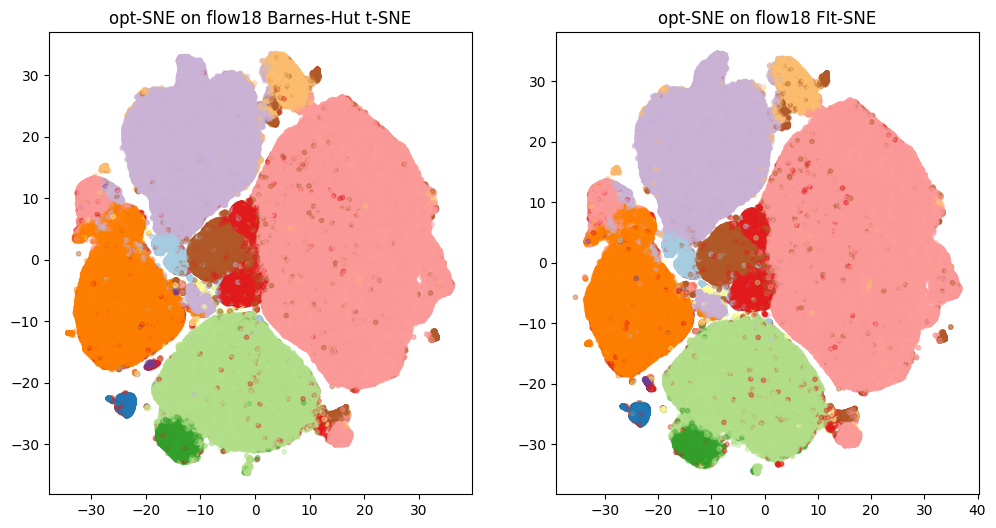
\includegraphics[width=\linewidth]{figures/BH_vs_FFT.png}
    \end{center}
\end{figure}
